% Sandia National Laboratories is a multimission laboratory managed and
% operated by National Technology & Engineering Solutions of Sandia, LLC, a
% wholly owned subsidiary of Honeywell International Inc., for the U.S.
% Department of Energy’s National Nuclear Security Administration under
% contract DE-NA0003525.

% Copyright 2002-2020 National Technology & Engineering Solutions of Sandia,
% LLC (NTESS).


%%
%% BJT Description Table
%%

\begin{Device}\label{Q_DEVICE}

\symbol
{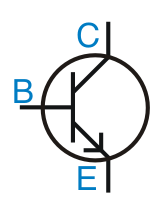
\includegraphics{npnSymbol}}
{
\includegraphics{pnpSymbol}}

\device
\begin{alltt}
Q<name> <collector node> <base node> <emitter node>
 + [substrate node] <model name> [area value]

Q<name> <collector node> <base node> <emitter node>
 + [thermal node] <VBIC 1.3 3-terminal model name>

Q<name> <collector node> <base node> <emitter node>
 + <substrate> [thermal node] <VBIC 1.3 4-terminal model name>

 Q<name> <collector node> <base node> <emitter node>
 + <substrate> <thermal node> <HICUM model name>
\end{alltt}

\model
\begin{alltt}
.MODEL <model name> NPN [model parameters]
.MODEL <model name> PNP [model parameters]
\end{alltt}

\examples
\begin{alltt}
Q2 10 2 9 PNP1
Q12 14 2 0 1 NPN2 2.0
Q6 VC 4 11 [SUB] LAXPNP
Q7 Coll Base Emit DT VBIC13MODEL2
Q8 Coll Base Emit VBIC13MODEL3 SW\_ET=0
Q9 Coll Base Emit Subst DT VBIC13MODEL4
Q10 Coll Base Emit Subst DT HICUMMMODEL1
\end{alltt}

\parameters
\begin{Parameters}
\param{substrate node}
  Optional and defaults to ground. Since \Xyce{} permits alphanumeric
  node names and because there is no easy way to make a distinction between
  these and the model names, the name (not a number) used for the substrate
  node must be enclosed in square brackets \texttt{[ ]}.  Otherwise, nodes
  would be interpreted as model names. See the fourth example above.

\param{area value}
  The relative device area with a default value of 1.

\end{Parameters}

\comments
The BJT is modeled as an intrinsic transistor using ohmic resistances in series
with the collector (RC/area), with the base (value varies with current, see BJT
equations) and with the emitter (RE/area).For model parameters with optional
names, such as VAF and VA (the optional name is in parentheses), either may be
used.For model types NPN and PNP, the isolation junction capacitance is
connected between the intrinsic-collector and substrate nodes. This is the same
as in SPICE and works well for vertical IC transistor structures.

\textbf{Only the VBIC 1.3 model is available in \Xyce{} 6.11 and
  later.}  The VBIC 1.3 model is provided in both 3-terminal (Q level
  11) and 4-terminal (Q level 12) variants, both supporting
  electrothermal and excess-phase effects.  These variants of the Q line
  are shown in the fourth through sixth examples above. VBIC 1.3
  instance lines have three or four required nodes, depending on model
  level, and an \emph{optional} ``dt'' node.  The first three are the
  normal collector, base,and emitter. In the level 12 (4-terminal) the
  fourth node is the substrate, just as for the level 1 BJT.  If the
  optional ``dt'' node is specified for either variant, it can be used
  to print the local temperature rise due to self-heating, and could
  possibly be used to model coupled heating effects of several VBIC
  devices.  It is, however, unnecessary to specify a ``dt'' node just
  to print the local temperature rise, because when this node is
  omitted from the instance line it simply becomes and internal node,
  and may still be printed using the syntax
  \texttt{N(instancename:dt)}.  For the ``Q8'' example above, one
  could print \texttt{N(Q8:dt)}.

As of release 6.10 of Xyce, the VBIC 1.3 3-terminal device (Q level
11) has been the subject of extensive optimization, and runs much
faster than in previous releases.

\textbf{ The HICUM models require both a substrate and thermal node.}

\end{Device}


% BJT model schematic.
\begin{figure}[ht]
  \centering
  \scalebox{0.6}
  {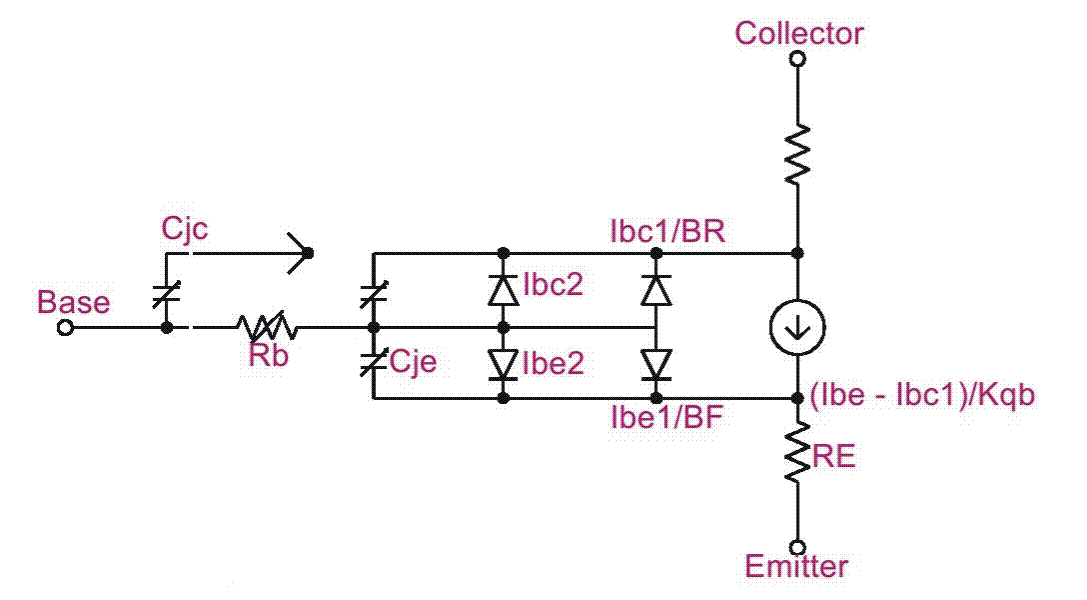
\includegraphics{bjtSchematic}}
  \caption[BJT model schematic]{BJT model schematic.  Adapted from
reference~\cite{PSpiceUG:1998}. \label{figBJTschematic}}
\end{figure}

\paragraph{BJT Level selection}

\Xyce{} supports the level 1 BJT model, which is based on the
documented standard SPICE 3F5 BJT model, but was coded independently
at Sandia.  It is mostly based on the classic Gummel-Poon BJT
model~\cite{GummelPoon}.

Two variants of the VBIC model are provided as BJT levels 11  and 12.
Levels 11 and 12 are the
3-terminal and 4-terminal variants of the VBIC 1.3.

An experimental release of the FBH HBT\_X model version
2.1\cite{Rudolph_documentationof} is provided as BJT level 23.

Both the HICUM/L0 (level 230) and HICUM/L2 (level 234) models are also
provided (\url{https://www.iee.et.tu-dresden.de/iee/eb/hic_new/hic_start.html}).

The MEXTRAM\cite{MEXTRAM_home} BJT model version 504.12.1 model is provided.
Two variants of this model are available: the level 504 model without
self-heating and without external substrate node, and the level 505 model with
self heating but without external substrate node.  The level 505 instance line
requires a fourth node for the 'dt' node, similar to the usage in all of the
VBIC models (levels 11-12), but is otherwise identical to the level 504 model.

\paragraph{BJT Power Calculations}
Power dissipated in the transistor is calculated with
$|I_{B}*V_{BE}|+|I_{C}*V_{CE}|$, where $I_{B}$ is the base current, $I_{C}$ is
the collector current, $V_{BE}$ is the voltage drop between the base and the
emitter and $V_{CE}$ is the voltage drop between the collector and the emitter.
This formula may differ from other simulators.

\subsubsection{The Level 1 Model}
\paragraph{BJT Equations}\label{bjt_equations}
The Level 1 BJT implementation within \Xyce{} is based on \cite{Fjeldly:1998}.
The equations in this section describe an NPN transistor. For the PNP device,
reverse the signs of all voltages and currents.  The equations use the
following variables:
%insert variables here
\begin{eqnarray*}
V_{be} & = & \mbox{intrinsic base-intrinsic emitter voltage} \\
V_{bc} & = & \mbox{intrinsic base-intrinsic collector voltage} \\
V_{bs} & = & \mbox{intrinsic base-substrate voltage} \\
V_{bw} & = & \mbox{intrinsic base-extrinsic collector voltage
(quasi-saturation only)} \\
V_{bx} & = & \mbox{extrinsic base-intrinsic collector voltage} \\
V_{ce} & = & \mbox{intrinsic collector-intrinsic emitter voltage} \\
V_{js} & = & \mbox{(NPN) intrinsic collector-substrate voltage} \\
&        = & \mbox{(PNP) intrinsic substrate-collector voltage} \\
% THIS DOESN'T EXIST IN XYCE
%&        = & \mbox{(LPNP) intrinsic base-substrate voltage} \\
V_{t}  & = & \mbox{$kT/q$ (thermal voltage)} \\
V_{th} & = & \mbox{threshold voltage} \\
k      & = & \mbox{Boltzmann's constant} \\
q      & = & \mbox{electron charge} \\
T      & = & \mbox{analysis temperature (K)} \\
T_{0}  & = & \mbox{nominal temperature (set using \textrmb{TNOM} option)}
\end{eqnarray*}
Other variables are listed above in BJT Model Parameters.

\subparagraph{DC Current}
The BJT model is based on the Gummel and Poon model~\cite{Grove:1967} where the
different terminal currents are written
%insert equations here
\begin{eqnarray*}
I_{e} & = & -I_{cc} - I_{be} + I_{re} + (C_{dife} +C_{de})\frac{dV_{be}}{dt} \\
I_{c} & = & -I_{cc} + I_{bc} - I_{rc} - (C_{difc}+ C_{dc})\frac{dV_{bc}}{dt} \\
I_b & = & I_e -I_c
\end{eqnarray*}
Here, $C_{dife}$ and $C_{difc}$ are the capacitances related to the hole
charges per unit area in the base, $Q_{dife}$ and $Q_{difc}$,
affiliated with the electrons introduced across the emitter-base and
collector-base junctions, respectively.  Also, $C_{be}$ and $C_{bc}$ are the
capacitances related to donations to the hole charge of the base, $Q_{be}$ and
$Q_{bc}$,  affiliated with the differences in the depletion regions of the
emitter-base and collector-base junctions, respectively.  The
intermediate currents used are defined as
%insert equations here
\begin{eqnarray*}
-I_{be} & = & \mathbf{\frac{IS}{BF}} \left[\exp \left(\frac{V_{be}}
{\mathbf{NF}V_{th}} \right) -1 \right] \\
-I_{cc} & = & \frac{Q_{bo}}{Q_{b}}\mathbf{IS} \left[\exp \left(\frac{V_{be}}
{\mathbf{NF} V_{th}} \right) -
\exp \left(\frac{V_{bc}}{\mathbf{NF}V_{th}} \right) \right] \\
-I_{bc} & = & \mathbf{\frac{IS}{BR}} \left[\exp \left(\frac{V_{bc}}
{\mathbf{NR}V_{th}} \right) - 1 \right] \\
I_{re} & = & \mathbf{ISE} \left[\exp \left(\frac{V_{be}}
{\mathbf{NE} V_{th}} \right) - 1 \right] \\
I_{rc} & = & \mathbf{ISC} \left[\exp \left(\frac{V_{bc}}
{\mathbf{NC}V_{th}} \right) - 1 \right]
\end{eqnarray*}
where the last two terms are the generation/recombination currents related to
the emitter and collector junctions, respectively.  The charge $Q_{b}$ is the
majority carrier charge in the base at large injection levels and is a key
difference in the Gummel-Poon model over the earlier Ebers-Moll model.  The
ratio $Q_b/Q_{bo}$ (where $Q_{bo}$ represents the zero-bias base charge, i.e.
the value of $Q_b$ when $V_{be}=V_{bc}=0$) as computed by \Xyce{} is given by
\[\frac{Q_b}{Q_{bo}} = \frac{q_1}{2}\left(1+\sqrt{1+4q_2}\right)\]
where
\begin{eqnarray*}
q_1 & = & \left(1-\frac{V_{be}}{\mathbf{VAR}}-\frac{V_{bc}}{\mathbf{VAF}}
\right)^{-1} \\
q_2 & = & \frac{\mathbf{IS}}{\mathbf{IKF}}\left[\exp\left(\frac{V_{be}}
{\mathbf{NF}V_{th}}\right)-1\right] + \frac{\mathbf{IS}}{\mathbf{IKR}}
\left[\exp\left(\frac{V_{bc}}{\mathbf{NR}V_{th}}\right)-1\right]
\end{eqnarray*}

\subparagraph{Capacitance Terms}
The capacitances listed in the above DC $I-V$ equations each consist of a
depletion layer capacitance $C_{d}$ and
a diffusion capacitance $C_{dif}$.  The first is given by
\[
C_d = \left\{
\begin{array}{ll}
\mathbf{CJ} \left(1 - \frac{V_{di}}{\mathbf{VJ}} \right)^{\mathbf{-M}} &
V_{di} \leq \mathbf{FC \cdot VJ} \\
\mathbf{CJ} \left(1 - \mathbf{FC} \right)^{-(1+\mathbf{M})} \
\left[1 - \mathbf{FC}(1 + \mathbf{M}) + \mathbf{M}
\frac{V_{di}}{\mathbf{VJ}} \right]
& V_{di} > \mathbf{FC \cdot VJ}
\end{array}
\right. \]

where $\mathbf{CJ}=\mathbf{CJE}$ for $C_{de}$, and where $\mathbf{CJ}=
\mathbf{CJC}$ for $C_{dc}$.
The diffusion capacitance (sometimes referred to as the transit time
capacitance) is
\[
C_{dif} = \mathbf{TT} G_d = \mathbf{TT} \frac{dI}{dV_{di}}
\]
where $I$ is the diode DC current given, $G_d$ is the corresponding junction
conductance, and where $\mathbf{TT}=\mathbf{TF}$ for $C_{dife}$ and
$\mathbf{TT}=\mathbf{TR}$ for $C_{difc}$.

\subparagraph{Temperature Effects}
SPICE temperature effects are default, but all levels of the BJT have a more
advanced temperature compensation available.  By specifying
\texttt{TEMPMODEL=QUADRATIC} in the netlist, parameters can be interpolated
quadratically between measured values extracted from data.  In the BJT, IS and
ISE are interpolated logarithmically because they can change over an order of
magnitude or more for temperature ranges of interest.  See the
Section~\ref{Model_Interpolation} for more details on how to include quadratic
temperature effects.

% \subparagraph{Noise}
% Noise is calculated with a 1.0 Hz bandwidth using the following spectral power
% densities (per unit bandwidth).

% Thermal Noise due to Parasitic Resistance: $I_{n}^{2} =
% \frac{4kT}{\mathbf{RS}/area}$

% Intrinsic Diode Shot and Flicker Noise: $I_{n}^{2} = 2qI_{D} +
% \mathbf{KF}\cdot\frac{I_{D}^{\mathbf{AF}}}{\omega}$

For further information on BJT models, see~\cite{Grove:1967}.  For a thorough
description of the U.C. Berkeley SPICE models see
Reference~\cite{Antognetti:1988}.

\subsubsection{VBIC Temperature Considerations}
\index{VBIC (temperature considerations)}
The VBIC (Q levels 11 and 12) model both support a self-heating
model.  The model works by computing the power dissipated by all
branches of the device, applying this power as a flow through a small
thermal network consisting of a power flow (``current'') source
through a thermal resistance and thermal capacitance, as shown in
Figure~\ref{vbicthermal}.  The circuit node DT will therefore be the
``thermal potential'' (temperature) across the parallel thermal
resistance and capacitance.  This temperature is the temperature rise
due to self heating of the device, which is added to the ambient
temperature and \texttt{TRISE} parameter to obtain the device
operating temperature.
\begin{figure}
  \centering
  \scalebox{0.3}
  {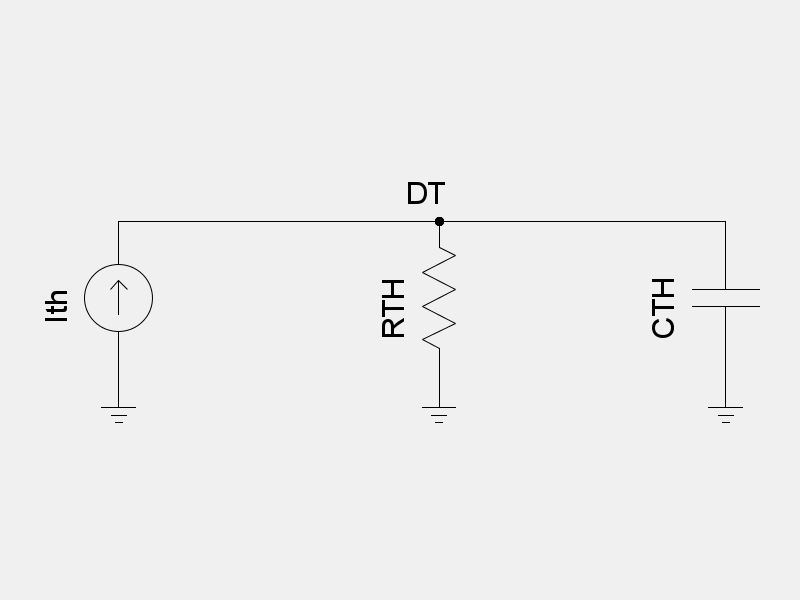
\includegraphics{VBIC_Thermal_Net}}
  \caption[VBIC thermal network schematic]{VBIC thermal network  schematic.}
  \label{vbicthermal}
\end{figure}

In VBIC 1.3, the dt node is optional on the netlist line.  If not
given, the dt node is used internally for thermal effects
calculations, but not accessible from the rest of the netlist.  The
VBIC 1.3 provides an instance parameter \texttt{SW\_ET} that may be
set to zero to turn off electrothermal self-heating effects.  When set
to zero, no thermal power is sourced into the dt node.  This parameter
defaults to 1, meaning that thermal power is computed and flows into
dt even when dt is unspecified on the netlist and remains an internal
node.

In VBIC 1.3, setting RTH to zero does {\em NOT\/} disable the
self-heating model, and does not short the dt node to ground, even
though one might expect that to be the behavior.  Rather, it simply
removes the RTH resistor from the equivalent circuit of
figure~\ref{vbicthermal} and leaves the dt node floating.  This is an
important point to recognize when using the VBIC.

If a node name is given as the fourth node of a VBIC \Xyce{} will emit
warnings about the node not having a DC path to ground and being
connected to only one device.  These warnings may safely be ignored,
and are a harmless artifact of Xyce's connectivity checker.  It is
possible to silence this warning by adding a very large resistance
between the dt node and ground --- 1GOhm or 1TOhm are effectively the
same as leaving the node floating, and will satisfy the connectivity
checker's tests.  This used to be the recommended means of silencing
the connectivity checker for the VBIC 1.2 where dt was a required
node, but it is safe {\em if and only if a nonzero\/} \texttt{RTH}
{\em value is specified for the device.}  If, however, RTH is zero,
then dt would otherwise be floating and your external resistance now
becomes the primary path for thermal power flow; rather than turning
off self-heating effects, it will be as if you had set RTH to a very
large value.  We therefore recommend that you not tie the dt node to
ground via a resistor, and if you are not using it to connect VBIC
devices together via a thermal network, simply leave off the dt node
to silence the connectivity checker warning.  Turn off self-heating
effects ONLY by setting the \texttt{SW\_ET} instance parameter to zero.

Users of earlier versions of \Xyce{} may have been using the VBIC 1.2
model that was removed in release 6.11.  All netlists containing the
old level=10 VBIC 1.2 model must be modified to run in \Xyce{} 6.11
and later.  The following points should be observed when converting an
old VBIC 1.2 netlist and model card to VBIC 1.3.

\begin{itemize}
  \item Generally speaking, most VBIC 1.2 model cards can be converted
    to VBIC 1.3 model cards by the simple substitution of
    \texttt{level=11} for \texttt{level=10}, with the following provisos.

  \item VBIC 1.2 in \Xyce{} 6.10 and earlier did not support excess
    phase effects, and so the \texttt{TD} parameter governing excess
    phase was ignored.

    The \Xyce{} team has observed that some users' VBIC 1.2 parameter
    extractions have a non-zero value for the \texttt{TD} parameter.
    The impact of this is twofold:
    \begin{itemize}
      \item Circuits that use such model cards with only the level
        number changed will likely not produce identical results when
        compared to simulation results of older versions of \Xyce{}
        using VBIC 1.2 due to the excess phase effects.  If strict
        comparison between VBIC 1.3 runs with \Xyce{} 6.11 or later
        against older runs with VBIC 1.2 is desired, change the
        \texttt{TD} parameter to zero.  This will disable the excess
        phase effects and make VBIC 1.3 equivalent to the VBIC 1.2
        that was previously provided.
      \item The \Xyce{} team has seen some instances where the
        previously ignored \texttt{TD} parameter value is such that
        \Xyce{} will fail to converge when the equivalent VBIC 1.3
        model is substituted.  The VBIC 1.2 behavior can be recovered
        by setting the model parameter \texttt{TD} to zero, which will
        disable the excess phase effect in VBIC 1.3.  We can only
        suggest that the model card be re-extracted using VBIC 1.3 to
        determine the correct value for \texttt{TD}.
    \end{itemize}

  \item VBIC 1.2 had a model parameter called \texttt{DTEMP}, which
    \Xyce{} also recognized on the instance line.  In VBIC 1.3 this
    parameter has been replaced by another called \texttt{TRISE},
    which is only an instance parameter, and is unrecognized in model
    cards.  VBIC 1.3 also recognizes \texttt{DTEMP} on the instance
    line as an alias for \texttt{TRISE}.  If you had been specifying
    \texttt{DTEMP} in your VBIC 1.2 model cards, you will need to move it
    to the instance line instead in order for the parameter to be
    properly recognized by both VBIC 1.2 and VBIC 1.3.
  \item Turning off self-heating effects in VBIC 1.2 was done by
    grounding the mandatory dt node.  This is not the recommended way
    of disabling self-heating in VBIC 1.3.  To disable self-heating,
    set the \texttt{SW\_ET} parameter to zero on the instance line (as
    is done in the ``Q8'' example above).
  \item If not using the dt node as a way of thermally coupling
    devices to each other, leave it off of VBIC 1.3 instance lines,
    allowing it to be an internal variable irrespective of whether
    self-heating is enabled or not.  This will silence any connectivity
    warnings from Xyce.  Since the dt node may be printed using the
    N() syntax even when internal, it is unnecessary to put a dt node
    on the instance line just to print the local temperature rise due
    to self-heating.  The only reasons to include it on the instance
    line would be for backward compatibility to VBIC 1.2 netlists, or
    to implement a thermal coupling network between devices.
  \item Finally, VBIC 1.3 introduced a number of constraints on model
    parameters that the previous version did not.  \Xyce{} will emit
    warnings if any parameter on a VBIC 1.3 model card is out of the
    range specified by the VBIC 1.3 authors.  These warnings should
    not be ignored lightly, as they indicate that the model is being
    used in a manner not intended by its authors.  They are generally
    a sign that the model may not be well-behaved, and may indicate an
    improperly extracted model card.

\end{itemize}

\subsubsection{Level 1 BJT Tables}
% This table was generated by Xyce:
%   Xyce -doc Q 1
%
\index{bipolar junction transistor!device instance parameters}
\begin{DeviceParamTableGenerated}{Bipolar Junction Transistor Device Instance Parameters}{Q_1_Device_Instance_Params}
AREA & Relative device area & -- & 1 \\ \hline
IC1 & Vector of initial values: Vbe,Vce. Vbe=IC1 & V & 0 \\ \hline
IC2 & Vector of initial values: Vbe,Vce. Vce=IC2 & V & 0 \\ \hline
LAMBERTW & Flag for toggling the use of the lambert-W function instead of exponentials. & logical (T/F) & false \\ \hline
OFF & Initial condition of no voltage drops accross device & logical (T/F) & false \\ \hline
TEMP & Device temperature & $^\circ$C & Ambient Temperature \\ \hline
\end{DeviceParamTableGenerated}

% This table was generated by Xyce:
%   Xyce -doc Q 1
%
\index{bipolar junction transistor!device model parameters}
\begin{DeviceParamTableGenerated}{Bipolar Junction Transistor Device Model Parameters}{Q_1_Device_Model_Params}
AF & Flicker noise exponent & --- & 1 \\ \hline
BF & Ideal maximum foward beta & -- & 100 \\ \hline
BFM & Ideal maximum foward beta & -- & 100 \\ \hline
BR & Ideal maximum reverse beta & -- & 1 \\ \hline
BRM & Ideal maximum reverse beta & -- & 1 \\ \hline
BV & Reverse early voltage & V & 0 \\ \hline
C2 & Coefficient for base-emitter leak current. & --- & 0 \\ \hline
C4 & Coefficient for base-collector leak current. & --- & 0 \\ \hline
CCS & Substrate zero-bias p-n capacitance & F & 0 \\ \hline
CDIS & Fraction of CJC connected internally to RB & -- & 1 \\ \hline
CJC & Base-collector zero-bias p-n capacitance & F & 0 \\ \hline
CJE & Base-emitter zero-bias p-n capacitance & F & 0 \\ \hline
CJS & Substrate zero-bias p-n capacitance & F & 0 \\ \hline
CSUB & Substrate zero-bias p-n capacitance & F & 0 \\ \hline
EG & Bandgap voltage (barrier highth) & eV & 1.11 \\ \hline
ESUB & Substrate p-n grading factor & -- & 0 \\ \hline
FC & Foward-bias depletion capacitor coefficient & -- & 0.5 \\ \hline
IK & Corner for foward-beta high-current roll-off & A & 0 \\ \hline
IKF & Corner for foward-beta high-current roll-off & A & 0 \\ \hline
IKR & Corner for reverse-beta high-current roll-off & A & 0 \\ \hline
IOB & Current at which RB falls off by half & A & 0 \\ \hline
IRB & Current at which RB falls off by half & A & 0 \\ \hline
IS & Transport saturation current & A & 1e-16 \\ \hline
ISC & Base-collector leakage saturation current & A & 0 \\ \hline
ISE & Base-emitter leakage saturation current & A & 0 \\ \hline
ITF & Transit time dependancy on IC & --- & 0 \\ \hline
JBF & Corner for foward-beta high-current roll-off & A & 0 \\ \hline
JBR & Corner for reverse-beta high-current roll-off & A & 0 \\ \hline
JLC & Base-collector leakage saturation current & A & 0 \\ \hline
JLE & Base-emitter leakage saturation current & A & 0 \\ \hline
JRB & Current at which RB falls off by half & A & 0 \\ \hline
JTF & Transit time dependancy on IC & --- & 0 \\ \hline
KF & Flicker noise coefficient & -- & 0 \\ \hline
MC & Base-collector p-n grading factor & -- & 0.33 \\ \hline
ME & Base-emitter p-n grading factor & -- & 0.33 \\ \hline
MJC & Base-collector p-n grading factor & -- & 0.33 \\ \hline
MJE & Base-emitter p-n grading factor & -- & 0.33 \\ \hline
MJS & Substrate p-n grading factor & -- & 0 \\ \hline
MS & Substrate p-n grading factor & -- & 0 \\ \hline
NC & Base-collector leakage emission coefficient & -- & 2 \\ \hline
NE & Base-emitter leakage emission coefficient & -- & 1.5 \\ \hline
NF & Foward current emission coefficient & -- & 1 \\ \hline
NK & High current rolloff coefficient & -- & 0.5 \\ \hline
NKF & High current rolloff coefficient & -- & 0.5 \\ \hline
NLE & Base-emitter leakage emission coefficient & -- & 1.5 \\ \hline
NR & Reverse current emission coefficient & -- & 1 \\ \hline
PC & Base-collector built-in potential & V & 0.75 \\ \hline
PE & Base-emitter built-in potential & V & 0.75 \\ \hline
PS & Substrate built-in potential & V & 0.75 \\ \hline
PSUB & Substrate built-in potential & V & 0.75 \\ \hline
PT & Temperature exponent for IS. (synonymous with XTI) & --- & 3 \\ \hline
PTF & Excess Phase at 1/(2pi*TF) Hz & degree & 0 \\ \hline
RB & Zero-bias (maximum) base resistance & $\mathsf{\Omega}$ & 0 \\ \hline
RBM & Maximum base resistance & $\mathsf{\Omega}$ & 0 \\ \hline
RC & Collector ohmic resistance & $\mathsf{\Omega}$ & 0 \\ \hline
RE & Emitter ohmic resistance & $\mathsf{\Omega}$ & 0 \\ \hline
TB & Foward and reverse beta temperature coefficient & -- & 0 \\ \hline
TCB & Foward and reverse beta temperature coefficient & -- & 0 \\ \hline
TEMPMODEL & Specifies the type of parameter interpolation over temperature & -- & 'NONE' \\ \hline
TF & Ideal foward transit time & s & 0 \\ \hline
TNOM & Parameter measurement temperature & $^\circ$C & Ambient Temperature \\ \hline
TR & Ideal reverse transit time & s & 0 \\ \hline
VA & Foward early voltage & V & 0 \\ \hline
VAF & Foward early voltage & V & 0 \\ \hline
VAR & Reverse early voltage & V & 0 \\ \hline
VB & Reverse early voltage & V & 0 \\ \hline
VBF & Foward early voltage & V & 0 \\ \hline
VJC & Base-collector built-in potential & V & 0.75 \\ \hline
VJE & Base-emitter built-in potential & V & 0.75 \\ \hline
VJS & Substrate built-in potential & V & 0.75 \\ \hline
VRB & Reverse early voltage & V & 0 \\ \hline
VTF & Transit time dependancy on Vbc & V & 0 \\ \hline
XCJC & Fraction of CJC connected internally to RB & -- & 1 \\ \hline
XTB & Foward and reverse beta temperature coefficient & -- & 0 \\ \hline
XTF & Transit time bias dependence coefficient & -- & 0 \\ \hline
XTI & Temperature exponent for IS. (synonymous with PT) & --- & 3 \\ \hline
\end{DeviceParamTableGenerated}


\subsubsection{Level 11 and 12 BJT Tables (VBIC 1.3)}
The VBIC 1.3 (level 11 transistor for 3-terminal, level 12 for
4-terminal) supports a number of instance parameters that are not
available in the VBIC 1.2.  The level 11 and level 12 differ only by
the number of required nodes.  The level 11 is the 3-terminal device,
having only collector, base, and emitter as required nodes.  The level
12 is the 4-terminal device, requiring collector, base, emitter and
substrate nodes.  Both models support an optional 'dt' node as their
last node on the instance line.

\textbf{Model cards extracted for the VBIC 1.2 will mostly work with the VBIC
1.3,  with one notable exception:} in VBIC 1.2 the \texttt{DTEMP} parameter was
a model parameter, and \Xyce{} allowed it also to be specified on the instance
line, overriding whatever was specified in the model.  This parameter was
replaced in VBIC 1.3 with the \texttt{TRISE} parameter, which is {\em only\/}
an instance parameter.  \texttt{DTEMP} and \texttt{DTA} are both supported as
aliases for the \texttt{TRISE} instance parameter.

% This table was generated by Xyce:
%   Xyce -doc Q 11
%
\index{vbic 1.3 3t!device instance parameters}
\begin{DeviceParamTableGenerated}{VBIC 1.3 3T Device Instance Parameters}{Q_11_Device_Instance_Params}
DTA &  Alias for trise & $^\circ$C & 0 \\ \hline
DTEMP &  Alias for trise & $^\circ$C & 0 \\ \hline
M & multiplicity factor & --- & 1 \\ \hline
OFF & Set to 1 to initialize device to OFF instead of normally & --- & 0 \\ \hline
SW\_ET & switch for self-heating:      0=no and 1=yes & --- & 1 \\ \hline
SW\_NOISE & switch for including noise:   0=no and 1=yes & --- & 1 \\ \hline
TRISE & local temperature delta to ambient (before self-heating) & $^\circ$C & 0 \\ \hline
\end{DeviceParamTableGenerated}

% This table was generated by Xyce:
%   Xyce -doc Q 11
%
\index{vbic 1.3 3t!device model parameters}
\begin{DeviceParamTableGenerated}{VBIC 1.3 3T Device Model Parameters}{Q_11_Device_Model_Params}
ABK & SiGe base current kink exponent & --- & 1 \\ \hline
AFN & b-e flicker noise current exponent & --- & 1 \\ \hline
AJC & b-c capacitance smoothing factor & --- & -0.5 \\ \hline
AJE & b-e capacitance smoothing factor & --- & -0.5 \\ \hline
AJS & c-s capacitance smoothing factor & --- & -0.5 \\ \hline
ART & smoothing parameter for reach-through & --- & 0.1 \\ \hline
AVC1 & b-c   weak avalanche parameter 1 & V$^{-1}$ & 0 \\ \hline
AVC2 & b-c   weak avalanche parameter 2 & --- & 0 \\ \hline
AVCX1 & bx-cx weak avalanche parameter 1 & V$^{-1}$ & 0 \\ \hline
AVCX2 & bx-cx weak avalanche parameter 2 & --- & 0 \\ \hline
BBK & SiGe base current kink current factor & A & 0 \\ \hline
BFN & b-e flicker noise 1/f exponent & --- & 1 \\ \hline
CBCO & extrinsic b-c overlap capacitance & F & 0 \\ \hline
CBEO & extrinsic b-e overlap capacitance & F & 0 \\ \hline
CCSO & extrinsic c-s overlap capacitance & F & 0 \\ \hline
CJC & zero-bias b-c depletion capacitance & F & 0 \\ \hline
CJCP & zero-bias extrinsic c-s depletion capacitance & F & 0 \\ \hline
CJE & zero-bias b-e depletion capacitance & F & 0 \\ \hline
CJEP & zero-bias extrinsic b-c depletion capacitance & F & 0 \\ \hline
CTH & thermal capacitance & --- & 0 \\ \hline
DEAR & delta activation energy for isrr & V & 0 \\ \hline
EA & activation energy for is & V & 1.12 \\ \hline
EAIC & activation energy for ibci and ibeip & V & 1.12 \\ \hline
EAIE & activation energy for ibei & V & 1.12 \\ \hline
EAIS & activation energy for ibcip & V & 1.12 \\ \hline
EANC & activation energy for ibcn and ibenp & V & 1.12 \\ \hline
EANE & activation energy for iben & V & 1.12 \\ \hline
EANS & activation energy for ibcnp & V & 1.12 \\ \hline
EAP & activation energy for isp & V & 1.12 \\ \hline
FC & forward bias depletion capacitance limit & --- & 0.9 \\ \hline
GAMM & epi doping parameter & --- & 0 \\ \hline
GMIN & minimum conductance & $\mathsf{\Omega}^{-1}$ & 1e-12 \\ \hline
HRCF & high current collector resistance factor & --- & 0 \\ \hline
IBBE & b-e   breakdown current & A & 1e-06 \\ \hline
IBCI & ideal b-c saturation current & A & 1e-16 \\ \hline
IBCIP & ideal parasitic b-c saturation current & A & 0 \\ \hline
IBCN & non-ideal b-c saturation current & A & 0 \\ \hline
IBCNP & non-ideal parasitic b-c saturation current & A & 0 \\ \hline
IBEI & ideal b-e saturation current & A & 1e-18 \\ \hline
IBEIP & ideal parasitic b-e saturation current & A & 0 \\ \hline
IBEN & non-ideal b-e saturation current & A & 0 \\ \hline
IBENP & non-ideal parasitic b-e saturation current & A & 0 \\ \hline
IBK0 & SiGe base current kink current reference & A & 0 \\ \hline
IKF & forward knee current  (zero=infinite) & A & 0 \\ \hline
IKP & parasitic knee current  (zero=infinite) & A & 0 \\ \hline
IKR & reverse knee current  (zero=infinite) & A & 0 \\ \hline
IS & transport saturation current & A & 1e-16 \\ \hline
ISP & parasitic transport saturation current & A & 0 \\ \hline
ISRR & ratio of is(reverse) to is(forward) & --- & 1 \\ \hline
ITF & tf coefficient of Ic dependence & A & 0 \\ \hline
KFN & b-e flicker noise constant & --- & 0 \\ \hline
MAXEXP & argument at which to linearize general exponentials & --- & 1e+22 \\ \hline
MC & b-c grading coefficient & --- & 0.33 \\ \hline
MCX & bx-cx grading coefficient for avalanche & --- & 0.33 \\ \hline
ME & b-e grading coefficient & --- & 0.33 \\ \hline
MS & c-s grading coefficient & --- & 0.33 \\ \hline
NBBE & b-e   breakdown emission coefficient & --- & 1 \\ \hline
NCI & ideal b-c emission coefficient & --- & 1 \\ \hline
NCIP & ideal parasitic b-c emission coefficient & --- & 1 \\ \hline
NCN & non-ideal b-c emission coefficient & --- & 2 \\ \hline
NCNP & non-ideal parasitic b-c emission coefficient & --- & 2 \\ \hline
NEI & ideal b-e emission coefficient & --- & 1 \\ \hline
NEN & non-ideal b-e emission coefficient & --- & 2 \\ \hline
NF & fwd emission coefficient (ideality factor) & --- & 1 \\ \hline
NFP & parasitic emission coeff (ideality factor) & --- & 1 \\ \hline
NKF & high current beta roll-off parameter & --- & 0.5 \\ \hline
NPN & npn transistor type & --- & 0 \\ \hline
NR & rev emission coefficient (ideality factor) & --- & 1 \\ \hline
OFF & Set to 1 to initialize device to OFF instead of normally & --- & 0 \\ \hline
PC & b-c built-in potential & V & 0.75 \\ \hline
PE & b-e built-in potential & V & 0.75 \\ \hline
PNJMAXI & current at which to linearize diode currents & A & 1 \\ \hline
PNP & pnp transistor type & --- & 0 \\ \hline
PS & c-s built-in potential & V & 0.75 \\ \hline
QBM & base charge model selection switch: 0=GP and 1=SGP & --- & 0 \\ \hline
QCO & epi charge parameter & C & 0 \\ \hline
QNIBEIR & ideal b-e quasi-neutral base recombination parameter & --- & 0 \\ \hline
QTF & variation of tf with base-width modulation & --- & 0 \\ \hline
RBI & intrinsic base resistance & $\mathsf{\Omega}$ & 0 \\ \hline
RBP & parasitic transistor base resistance & $\mathsf{\Omega}$ & 0 \\ \hline
RBX & extrinsic base resistance & $\mathsf{\Omega}$ & 0 \\ \hline
RCI & intrinsic collector resistance & $\mathsf{\Omega}$ & 0 \\ \hline
RCX & extrinsic collector resistance & $\mathsf{\Omega}$ & 0 \\ \hline
RE & extrinsic emitter resistance & $\mathsf{\Omega}$ & 0 \\ \hline
RS & extrinsic substrate resistance & $\mathsf{\Omega}$ & 0 \\ \hline
RTH & thermal resistance & --- & 0 \\ \hline
SCALE & scale  factor for instance geometries & --- & 1 \\ \hline
SHRINK & shrink percentage for instance geometries & --- & 0 \\ \hline
TAVC & temperature exponent of avc2 & $^\circ$C$^{-1}$ & 0 \\ \hline
TAVCX & temperature exponent of avcx2 & $^\circ$C$^{-1}$ & 0 \\ \hline
TCRTH & temperature exponent of rth & $^\circ$C$^{-1}$ & 0 \\ \hline
TCVEF & temperature exponent of vef & $^\circ$C$^{-1}$ & 0 \\ \hline
TCVER & temperature exponent of ver & $^\circ$C$^{-1}$ & 0 \\ \hline
TD & forward excess-phase delay time & s & 0 \\ \hline
TF & forward transit time & s & 0 \\ \hline
TMAX & maximum ambient temperature & $^\circ$C & 500 \\ \hline
TMAXCLIP & clip maximum temperature & $^\circ$C & 500 \\ \hline
TMIN & minimum ambient temperature & $^\circ$C & -100 \\ \hline
TMINCLIP & clip minimum temperature & $^\circ$C & -100 \\ \hline
TNBBE & temperature coefficient of nbbe & $^\circ$C$^{-1}$ & 0 \\ \hline
TNF & temperature exponent of nf and nr & $^\circ$C$^{-1}$ & 0 \\ \hline
TNOM & nominal (reference) temperature & $^\circ$C & 27 \\ \hline
TR & reverse transit time & s & 0 \\ \hline
TVBBE1 & linear temperature coefficient of vbbe & $^\circ$C$^{-1}$ & 0 \\ \hline
TVBBE2 & quadratic temperature coefficient of vbbe & --- & 0 \\ \hline
TYPE & transistor type: -1=npn and +1=pnp (overriden by npn or pnp) & --- & -1 \\ \hline
VBBE & b-e   breakdown voltage & V & 0 \\ \hline
VEF & forward Early voltage (zero=infinite) & V & 0 \\ \hline
VER & reverse Early voltage (zero=infinite) & V & 0 \\ \hline
VO & epi drift saturation voltage & V & 0 \\ \hline
VPTE & SiGe base current kink voltage & V & 0 \\ \hline
VRT & reach-through voltage for Cbc limiting & V & 0 \\ \hline
VTF & tf coefficient of Vbci dependence & V & 0 \\ \hline
WBE & partitioning of Ibe/Ibex and Qbe/Qbex & --- & 1 \\ \hline
WSP & partitioning of Iccp between Vbep and Vbci & --- & 1 \\ \hline
XII & temperature exponent of ibei, ibci, ibeip, ibcip & --- & 3 \\ \hline
XIKF & temperature exponent of ikf & --- & 0 \\ \hline
XIN & temperature exponent of iben, ibcn, ibenp, ibcnp & --- & 3 \\ \hline
XIS & temperature exponent of is & --- & 3 \\ \hline
XISR & temperature exponent for isrr & --- & 0 \\ \hline
XRB & temperature exponent of rbx and rbi & --- & 0 \\ \hline
XRBI & temperature exponent of rbi (overrides xrb) & --- & 0 \\ \hline
XRBP & temperature exponent of rbp (overrides xrc) & --- & 0 \\ \hline
XRBX & temperature exponent of rbx (overrides xrb) & --- & 0 \\ \hline
XRC & temperature exponent of rci and rcx and rbp & --- & 0 \\ \hline
XRCI & temperature exponent of rci (overrides xrc) & --- & 0 \\ \hline
XRCX & temperature exponent of rcx (overrides xrc) & --- & 0 \\ \hline
XRE & temperature exponent of re & --- & 0 \\ \hline
XRS & temperature exponent of rs & --- & 0 \\ \hline
XTF & tf bias dependence coefficient & --- & 0 \\ \hline
XVO & temperature exponent of vo & --- & 0 \\ \hline
\end{DeviceParamTableGenerated}

\clearpage
% This table was generated by Xyce:
%   Xyce -doc Q 12
%
\index{vbic 1.3 4t!device instance parameters}
\begin{DeviceParamTableGenerated}{VBIC 1.3 4T Device Instance Parameters}{Q_12_Device_Instance_Params}
DTA &  Alias for trise & $^\circ$C & 0 \\ \hline
DTEMP &  Alias for trise & $^\circ$C & 0 \\ \hline
M & multiplicity factor & --- & 1 \\ \hline
OFF & Set to 1 to initialize device to OFF instead of normally & --- & 0 \\ \hline
SW\_ET & switch for self-heating:      0=no and 1=yes & --- & 1 \\ \hline
SW\_NOISE & switch for including noise:   0=no and 1=yes & --- & 1 \\ \hline
TRISE & local temperature delta to ambient (before self-heating) & $^\circ$C & 0 \\ \hline
\end{DeviceParamTableGenerated}

% This table was generated by Xyce:
%   Xyce -doc Q 12
%
\index{vbic 1.3 4t!device model parameters}
\begin{DeviceParamTableGenerated}{VBIC 1.3 4T Device Model Parameters}{Q_12_Device_Model_Params}
ABK & SiGe base current kink exponent & --- & 1 \\ \hline
AFN & b-e flicker noise current exponent & --- & 1 \\ \hline
AJC & b-c capacitance smoothing factor & --- & -0.5 \\ \hline
AJE & b-e capacitance smoothing factor & --- & -0.5 \\ \hline
AJS & c-s capacitance smoothing factor & --- & -0.5 \\ \hline
ART & smoothing parameter for reach-through & --- & 0.1 \\ \hline
AVC1 & b-c   weak avalanche parameter 1 & V$^{-1}$ & 0 \\ \hline
AVC2 & b-c   weak avalanche parameter 2 & --- & 0 \\ \hline
AVCX1 & bx-cx weak avalanche parameter 1 & V$^{-1}$ & 0 \\ \hline
AVCX2 & bx-cx weak avalanche parameter 2 & --- & 0 \\ \hline
BBK & SiGe base current kink current factor & A & 0 \\ \hline
BFN & b-e flicker noise 1/f exponent & --- & 1 \\ \hline
CBCO & extrinsic b-c overlap capacitance & F & 0 \\ \hline
CBEO & extrinsic b-e overlap capacitance & F & 0 \\ \hline
CCSO & extrinsic c-s overlap capacitance & F & 0 \\ \hline
CJC & zero-bias b-c depletion capacitance & F & 0 \\ \hline
CJCP & zero-bias extrinsic c-s depletion capacitance & F & 0 \\ \hline
CJE & zero-bias b-e depletion capacitance & F & 0 \\ \hline
CJEP & zero-bias extrinsic b-c depletion capacitance & F & 0 \\ \hline
CTH & thermal capacitance & --- & 0 \\ \hline
DEAR & delta activation energy for isrr & V & 0 \\ \hline
EA & activation energy for is & V & 1.12 \\ \hline
EAIC & activation energy for ibci and ibeip & V & 1.12 \\ \hline
EAIE & activation energy for ibei & V & 1.12 \\ \hline
EAIS & activation energy for ibcip & V & 1.12 \\ \hline
EANC & activation energy for ibcn and ibenp & V & 1.12 \\ \hline
EANE & activation energy for iben & V & 1.12 \\ \hline
EANS & activation energy for ibcnp & V & 1.12 \\ \hline
EAP & activation energy for isp & V & 1.12 \\ \hline
FC & forward bias depletion capacitance limit & --- & 0.9 \\ \hline
GAMM & epi doping parameter & --- & 0 \\ \hline
GMIN & minimum conductance & $\mathsf{\Omega}^{-1}$ & 1e-12 \\ \hline
HRCF & high current collector resistance factor & --- & 0 \\ \hline
IBBE & b-e   breakdown current & A & 1e-06 \\ \hline
IBCI & ideal b-c saturation current & A & 1e-16 \\ \hline
IBCIP & ideal parasitic b-c saturation current & A & 0 \\ \hline
IBCN & non-ideal b-c saturation current & A & 0 \\ \hline
IBCNP & non-ideal parasitic b-c saturation current & A & 0 \\ \hline
IBEI & ideal b-e saturation current & A & 1e-18 \\ \hline
IBEIP & ideal parasitic b-e saturation current & A & 0 \\ \hline
IBEN & non-ideal b-e saturation current & A & 0 \\ \hline
IBENP & non-ideal parasitic b-e saturation current & A & 0 \\ \hline
IBK0 & SiGe base current kink current reference & A & 0 \\ \hline
IKF & forward knee current  (zero=infinite) & A & 0 \\ \hline
IKP & parasitic knee current  (zero=infinite) & A & 0 \\ \hline
IKR & reverse knee current  (zero=infinite) & A & 0 \\ \hline
IS & transport saturation current & A & 1e-16 \\ \hline
ISP & parasitic transport saturation current & A & 0 \\ \hline
ISRR & ratio of is(reverse) to is(forward) & --- & 1 \\ \hline
ITF & tf coefficient of Ic dependence & A & 0 \\ \hline
KFN & b-e flicker noise constant & --- & 0 \\ \hline
MAXEXP & argument at which to linearize general exponentials & --- & 1e+22 \\ \hline
MC & b-c grading coefficient & --- & 0.33 \\ \hline
MCX & bx-cx grading coefficient for avalanche & --- & 0.33 \\ \hline
ME & b-e grading coefficient & --- & 0.33 \\ \hline
MS & c-s grading coefficient & --- & 0.33 \\ \hline
NBBE & b-e   breakdown emission coefficient & --- & 1 \\ \hline
NCI & ideal b-c emission coefficient & --- & 1 \\ \hline
NCIP & ideal parasitic b-c emission coefficient & --- & 1 \\ \hline
NCN & non-ideal b-c emission coefficient & --- & 2 \\ \hline
NCNP & non-ideal parasitic b-c emission coefficient & --- & 2 \\ \hline
NEI & ideal b-e emission coefficient & --- & 1 \\ \hline
NEN & non-ideal b-e emission coefficient & --- & 2 \\ \hline
NF & fwd emission coefficient (ideality factor) & --- & 1 \\ \hline
NFP & parasitic emission coeff (ideality factor) & --- & 1 \\ \hline
NKF & high current beta roll-off parameter & --- & 0.5 \\ \hline
NPN & npn transistor type & --- & 0 \\ \hline
NR & rev emission coefficient (ideality factor) & --- & 1 \\ \hline
OFF & Set to 1 to initialize device to OFF instead of normally & --- & 0 \\ \hline
PC & b-c built-in potential & V & 0.75 \\ \hline
PE & b-e built-in potential & V & 0.75 \\ \hline
PNJMAXI & current at which to linearize diode currents & A & 1 \\ \hline
PNP & pnp transistor type & --- & 0 \\ \hline
PS & c-s built-in potential & V & 0.75 \\ \hline
QBM & base charge model selection switch: 0=GP and 1=SGP & --- & 0 \\ \hline
QCO & epi charge parameter & C & 0 \\ \hline
QNIBEIR & ideal b-e quasi-neutral base recombination parameter & --- & 0 \\ \hline
QTF & variation of tf with base-width modulation & --- & 0 \\ \hline
RBI & intrinsic base resistance & $\mathsf{\Omega}$ & 0 \\ \hline
RBP & parasitic transistor base resistance & $\mathsf{\Omega}$ & 0 \\ \hline
RBX & extrinsic base resistance & $\mathsf{\Omega}$ & 0 \\ \hline
RCI & intrinsic collector resistance & $\mathsf{\Omega}$ & 0 \\ \hline
RCX & extrinsic collector resistance & $\mathsf{\Omega}$ & 0 \\ \hline
RE & extrinsic emitter resistance & $\mathsf{\Omega}$ & 0 \\ \hline
RS & extrinsic substrate resistance & $\mathsf{\Omega}$ & 0 \\ \hline
RTH & thermal resistance & --- & 0 \\ \hline
SCALE & scale  factor for instance geometries & --- & 1 \\ \hline
SHRINK & shrink percentage for instance geometries & --- & 0 \\ \hline
TAVC & temperature exponent of avc2 & $^\circ$C$^{-1}$ & 0 \\ \hline
TAVCX & temperature exponent of avcx2 & $^\circ$C$^{-1}$ & 0 \\ \hline
TCRTH & temperature exponent of rth & $^\circ$C$^{-1}$ & 0 \\ \hline
TCVEF & temperature exponent of vef & $^\circ$C$^{-1}$ & 0 \\ \hline
TCVER & temperature exponent of ver & $^\circ$C$^{-1}$ & 0 \\ \hline
TD & forward excess-phase delay time & s & 0 \\ \hline
TF & forward transit time & s & 0 \\ \hline
TMAX & maximum ambient temperature & $^\circ$C & 500 \\ \hline
TMAXCLIP & clip maximum temperature & $^\circ$C & 500 \\ \hline
TMIN & minimum ambient temperature & $^\circ$C & -100 \\ \hline
TMINCLIP & clip minimum temperature & $^\circ$C & -100 \\ \hline
TNBBE & temperature coefficient of nbbe & $^\circ$C$^{-1}$ & 0 \\ \hline
TNF & temperature exponent of nf and nr & $^\circ$C$^{-1}$ & 0 \\ \hline
TNOM & nominal (reference) temperature & $^\circ$C & 27 \\ \hline
TR & reverse transit time & s & 0 \\ \hline
TVBBE1 & linear temperature coefficient of vbbe & $^\circ$C$^{-1}$ & 0 \\ \hline
TVBBE2 & quadratic temperature coefficient of vbbe & --- & 0 \\ \hline
TYPE & transistor type: -1=npn and +1=pnp (overriden by npn or pnp) & --- & -1 \\ \hline
VBBE & b-e   breakdown voltage & V & 0 \\ \hline
VEF & forward Early voltage (zero=infinite) & V & 0 \\ \hline
VER & reverse Early voltage (zero=infinite) & V & 0 \\ \hline
VO & epi drift saturation voltage & V & 0 \\ \hline
VPTE & SiGe base current kink voltage & V & 0 \\ \hline
VRT & reach-through voltage for Cbc limiting & V & 0 \\ \hline
VTF & tf coefficient of Vbci dependence & V & 0 \\ \hline
WBE & partitioning of Ibe/Ibex and Qbe/Qbex & --- & 1 \\ \hline
WSP & partitioning of Iccp between Vbep and Vbci & --- & 1 \\ \hline
XII & temperature exponent of ibei, ibci, ibeip, ibcip & --- & 3 \\ \hline
XIKF & temperature exponent of ikf & --- & 0 \\ \hline
XIN & temperature exponent of iben, ibcn, ibenp, ibcnp & --- & 3 \\ \hline
XIS & temperature exponent of is & --- & 3 \\ \hline
XISR & temperature exponent for isrr & --- & 0 \\ \hline
XRB & temperature exponent of rbx and rbi & --- & 0 \\ \hline
XRBI & temperature exponent of rbi (overrides xrb) & --- & 0 \\ \hline
XRBP & temperature exponent of rbp (overrides xrc) & --- & 0 \\ \hline
XRBX & temperature exponent of rbx (overrides xrb) & --- & 0 \\ \hline
XRC & temperature exponent of rci and rcx and rbp & --- & 0 \\ \hline
XRCI & temperature exponent of rci (overrides xrc) & --- & 0 \\ \hline
XRCX & temperature exponent of rcx (overrides xrc) & --- & 0 \\ \hline
XRE & temperature exponent of re & --- & 0 \\ \hline
XRS & temperature exponent of rs & --- & 0 \\ \hline
XTF & tf bias dependence coefficient & --- & 0 \\ \hline
XVO & temperature exponent of vo & --- & 0 \\ \hline
\end{DeviceParamTableGenerated}

\clearpage

\subsubsection{Level 23 BJT Tables (FBH HBT\_X)}
% This table was generated by Xyce:
%   Xyce -doc Q 23
%
\index{fbh hbtx v2.1!device instance parameters}
\begin{DeviceParamTableGenerated}{FBH HBT\_\-X v2.1 Device Instance Parameters}{Q_23_Device_Instance_Params}
L & Length of emitter fingers & m & 3e-05 \\ \hline
N & Number of emitter fingers & -- & 1 \\ \hline
TEMP & Device operating temperature & $^\circ$C & 25 \\ \hline
W & Width of emitter fingers & m & 3e-06 \\ \hline
\end{DeviceParamTableGenerated}

% This table was generated by Xyce:
%   Xyce -doc Q 23
%
\index{fbh hbtx v2.1!device model parameters}
\begin{DeviceParamTableGenerated}{FBH HBT\_\-X v2.1 Device Model Parameters}{Q_23_Device_Model_Params}
AHC &  & -- & 0 \\ \hline
BF &  & -- & 100 \\ \hline
BR &  & -- & 1 \\ \hline
BVCEO &  & -- & 0 \\ \hline
BVEBO &  & -- & 0 \\ \hline
CJC &  & -- & 1e-15 \\ \hline
CJE &  & -- & 1e-15 \\ \hline
CMIN &  & -- & 1e-16 \\ \hline
CPB &  & -- & 0 \\ \hline
CPC &  & -- & 0 \\ \hline
CQ &  & -- & 0 \\ \hline
CTH &  & -- & 7e-07 \\ \hline
DEBUG &  & -- & 0 \\ \hline
DEBUGPLUS &  & -- & 0 \\ \hline
IKF &  & -- & 0 \\ \hline
IKR &  & -- & 0 \\ \hline
J0 &  & -- & 0.001 \\ \hline
JK &  & -- & 0.0004 \\ \hline
JSC &  & -- & 0 \\ \hline
JSE &  & -- & 0 \\ \hline
JSEE &  & -- & 0 \\ \hline
JSF &  & -- & 2e-23 \\ \hline
JSR &  & -- & 2e-17 \\ \hline
KBETA &  & -- & 0 \\ \hline
KC &  & -- & 0 \\ \hline
KJC &  & -- & 1 \\ \hline
L & Length of emitter fingers & m & 3e-05 \\ \hline
LB &  & -- & 0 \\ \hline
LC &  & -- & 0 \\ \hline
LE &  & -- & 0 \\ \hline
MC &  & -- & 0 \\ \hline
MJC &  & -- & 0.5 \\ \hline
MJE &  & -- & 0.5 \\ \hline
MODE &  & -- & 1 \\ \hline
N & Number of emitter fingers & -- & 1 \\ \hline
NC &  & -- & 0 \\ \hline
NE &  & -- & 0 \\ \hline
NEE &  & -- & 0 \\ \hline
NF &  & -- & 1 \\ \hline
NOISE &  & -- & 1 \\ \hline
NR &  & -- & 1 \\ \hline
RB &  & -- & 1 \\ \hline
RB2 &  & -- & 1 \\ \hline
RBBXX &  & -- & 1e+06 \\ \hline
RBXX &  & -- & 1e+06 \\ \hline
RC &  & -- & 1 \\ \hline
RCI0 &  & -- & 0.001 \\ \hline
RCXX &  & -- & 1e+06 \\ \hline
RE &  & -- & 1 \\ \hline
RJK &  & -- & 0.001 \\ \hline
RTH &  & -- & 0.1 \\ \hline
TEMP & Device operating temperature & $^\circ$C & 25 \\ \hline
TF &  & -- & 1e-12 \\ \hline
TFT &  & -- & 0 \\ \hline
THCS &  & -- & 0 \\ \hline
TNOM &  & -- & 20 \\ \hline
TR &  & -- & 1e-15 \\ \hline
TRX &  & -- & 1e-15 \\ \hline
VAF &  & -- & 0 \\ \hline
VAR &  & -- & 0 \\ \hline
VCES &  & -- & 0.001 \\ \hline
VG &  & -- & 1.3 \\ \hline
VGB &  & -- & 0 \\ \hline
VGBB &  & -- & 0 \\ \hline
VGC &  & -- & 0 \\ \hline
VGR &  & -- & 0 \\ \hline
VJC &  & -- & 1.3 \\ \hline
VJE &  & -- & 1.3 \\ \hline
W & Width of emitter fingers & m & 3e-06 \\ \hline
XCJC &  & -- & 0.5 \\ \hline
XJ0 &  & -- & 1 \\ \hline
\end{DeviceParamTableGenerated}

\clearpage

\subsubsection{Level 230 BJT Tables (HICUM/L0)}
% This table was generated by Xyce:
%   Xyce -doc_cat Q 230
%
\index{hicum l0 v1.32!device instance parameters}
\begin{DeviceParamTableGenerated}{HICUM L0 v1.32 Device Instance Parameters}{Q_230_Device_Instance_Params}
DT & Temperature change for particular transistor & -- & 0 \\ \hline
\end{DeviceParamTableGenerated}

% This table was generated by Xyce:
%   Xyce -doc_cat Q 230
%
\index{hicum l0 v1.32!device model parameters}
\begin{DeviceParamTableGenerated}{HICUM L0 v1.32 Device Model Parameters}{Q_230_Device_Model_Params}
AF & flicker noise exponent factor & -- & 2 \\ \hline
AHC & Smoothing facor for current dependence & -- & 0.1 \\ \hline
AHQ & Smoothing factor for the d.c. injection width & -- & 0 \\ \hline
AJE & Ratio of maximum to zero-bias value & -- & 2.5 \\ \hline
AJEDC & BE capacitance ratio Ratio maximum to zero-bias value for d.c. transfer current & -- & 2.5 \\ \hline
ALCES & Relative TC of vces & -- & 0 \\ \hline
ALEAV & TC of avalanche exponential factor & -- & 0 \\ \hline
ALIQFH & Frist-order TC of iqfh & -- & 0 \\ \hline
ALIT & Factor for additional delay time of transfer current & -- & 0.333 \\ \hline
ALKAV & TC of avalanche prefactor & -- & 0 \\ \hline
ALQF & Factor for additional delay time of minority charge & -- & 0.167 \\ \hline
ALT0 & Frist-order TC of tf0 & -- & 0 \\ \hline
ALVS & Relative TC of satur.drift velocity & -- & 0 \\ \hline
AVER & bias dependence for reverse Early voltage & -- & 0 \\ \hline
CBCPAR & Collector-base isolation (overlap) capacitance & -- & 0 \\ \hline
CBEPAR & Emitter-base oxide capacitance & -- & 0 \\ \hline
CJCI0 & Total zero-bias BC depletion capacitance & -- & 1e-20 \\ \hline
CJCX0 & Zero-bias external BC depletion capacitance & -- & 1e-20 \\ \hline
CJE0 & Zero-bias BE depletion capacitance & -- & 1e-20 \\ \hline
CJS0 & Zero-bias SC depletion capacitance & -- & 1e-20 \\ \hline
CTH & Thermal capacitance & -- & 0 \\ \hline
DT0H &  & -- & 0 \\ \hline
DVGBE & Bandgap difference between base and BE-junction & -- & 0 \\ \hline
EAVL & Exponent factor & -- & 0 \\ \hline
F1VG & Coefficient K1 in T-dependent bandgap equation & -- & -0.000102377 \\ \hline
F2VG & Coefficient K2 in T-dependent bandgap equation & -- & 0.00043215 \\ \hline
FBC & Split factor = Cjci0/Cjc0 & -- & 1 \\ \hline
FGEO & Geometry factor & -- & 0.656 \\ \hline
FIQF & flag for turning on base related critical current & -- & 0 \\ \hline
FLNQS & Flag for turning on and off of vertical NQS effect & -- & 0 \\ \hline
FLSH & Flag for self-heating calculation & -- & 0 \\ \hline
GTE & Exponent factor for emmiter transit time & -- & 1 \\ \hline
IBCS & BC saturation current & -- & 0 \\ \hline
IBES & BE saturation current & -- & 1e-18 \\ \hline
IQF & forward d.c. high-injection toll-off current & -- & 1e+06 \\ \hline
IQFH & high-injection correction current & -- & 1e+06 \\ \hline
IQR & inverse d.c. high-injection roll-off current & -- & 1e+06 \\ \hline
IRES & BE recombination saturation current & -- & 0 \\ \hline
IS & (Modified) saturation current & -- & 1e-16 \\ \hline
ISCS & SC saturation current & -- & 0 \\ \hline
IT\_MOD & Flag for using third order solution for transfer current & -- & 0 \\ \hline
ITSS & Substrate transistor transfer saturation current & -- & 0 \\ \hline
KAVL & Prefactor & -- & 0 \\ \hline
KF & flicker noise coefficient & -- & 0 \\ \hline
KIQFH & Second-order TC of iqfh & -- & 0 \\ \hline
KT0 & Second-order TC of tf0 & -- & 0 \\ \hline
MBC & BC non-ideality factor & -- & 1 \\ \hline
MBE & BE non-ideality factor & -- & 1 \\ \hline
MCF & Non-ideality coefficient of forward collector current & -- & 1 \\ \hline
MCR & Non-ideality coefficient of reverse collector current & -- & 1 \\ \hline
MRE & BE recombination non-ideality factor & -- & 2 \\ \hline
MSC & SC non-ideality factor & -- & 1 \\ \hline
MSF & Substrate transistor transfer current non-ideality factor & -- & 1 \\ \hline
RBI0 & Internal base resistance at zero-bias & -- & 0 \\ \hline
RBX & External base series resistance & -- & 0 \\ \hline
RCI0 & Low-field collector resistance under emitter & -- & 150 \\ \hline
RCX & Emitter series resistance & -- & 0 \\ \hline
RE & External collector series resistance & -- & 0 \\ \hline
RTH & Thermal resistance & -- & 0 \\ \hline
T0 & low current transit time at Vbici=0 & -- & 0 \\ \hline
TBVL & SCR width modulation contribution & -- & 0 \\ \hline
TEF0 & Storage time in neutral emitter & -- & 0 \\ \hline
TEF\_TEMP & Flag for turning temperature dependence of tef0 on and off & -- & 1 \\ \hline
TFH & high-injection correction factor & -- & 0 \\ \hline
THCS & Saturation time at high current densities & -- & 0 \\ \hline
TNOM & Temperature for which parameters are valid & -- & 27 \\ \hline
TR & Storage time at inverse operation & -- & 0 \\ \hline
TYPE & For transistor type NPN(+1) or PNP (-1) & -- & 1 \\ \hline
VCES & Saturation voltage & -- & 0.1 \\ \hline
VDCI & BC built-in voltage & -- & 0.7 \\ \hline
VDCX & External BC built-in voltage & -- & 0.7 \\ \hline
VDE & BE built-in voltage & -- & 0.9 \\ \hline
VDEDC & BE charge built-in voltage for d.c. transfer current & -- & 0.9 \\ \hline
VDS & SC built-in voltage & -- & 0.3 \\ \hline
VEF & forward Early voltage (normalization volt.) & -- & 1e+06 \\ \hline
VER & reverse Early voltage (normalization volt.) & -- & 1e+06 \\ \hline
VGB & Bandgap-voltage & -- & 1.2 \\ \hline
VGC & Effective collector bandgap-voltage & -- & 1.17 \\ \hline
VGE & Effective emitter bandgap-voltage & -- & 1.17 \\ \hline
VGS & Effective substrate bandgap-voltage & -- & 1.17 \\ \hline
VLIM & Voltage dividing ohmic and satur.region & -- & 0.5 \\ \hline
VPT & Punch-through voltage & -- & 100 \\ \hline
VPTCI & Punch-through voltage of BC junction & -- & 100 \\ \hline
VPTCX & Punch-through voltage & -- & 100 \\ \hline
VPTS & SC punch-through voltage & -- & 100 \\ \hline
VR0C & forward Early voltage (normalization volt.) & -- & 1e+06 \\ \hline
VR0E & forward Early voltage (normalization volt.) & -- & 2.5 \\ \hline
ZCI & BC exponent factor & -- & 0.333 \\ \hline
ZCX & External BC exponent factor & -- & 0.333 \\ \hline
ZE & BE exponent factor & -- & 0.5 \\ \hline
ZEDC & charge BE exponent factor for d.c. transfer current & -- & 0.5 \\ \hline
ZETABET & Exponent coefficient in BE junction current temperature dependence & -- & 3.5 \\ \hline
ZETACI & TC of epi-collector diffusivity & -- & 0 \\ \hline
ZETACT & Exponent coefficient in transfer current temperature dependence & -- & 3 \\ \hline
ZETAIQF & TC of iqf & -- & 0 \\ \hline
ZETARBI & TC of internal base resistance & -- & 0 \\ \hline
ZETARBX & TC of external base resistance & -- & 0 \\ \hline
ZETARCX & TC of external collector resistance & -- & 0 \\ \hline
ZETARE & TC of emitter resistances & -- & 0 \\ \hline
ZETARTH & Exponent factor for temperature dependent thermal resistance & -- & 0 \\ \hline
ZETAVER & TC of Reverse Early voltage & -- & -1 \\ \hline
ZETAVGBE & TC of AVER & -- & 1 \\ \hline
ZS & External SC exponent factor & -- & 0.3 \\ \hline
\end{DeviceParamTableGenerated}

\clearpage

\subsubsection{Level 234 BJT Table (HICUM/L2)}
\textbf{NOTE:} The HICUM/L2 model has no instance parameters.
% This table was generated by Xyce:
%   Xyce -doc Q 234
%
\index{hicum v2.4.0!device model parameters}
\begin{DeviceParamTableGenerated}{HICUM v2.4.0 Device Model Parameters}{Q_234_Device_Model_Params}
ABET & Exponent factor for tunneling current & -- & 40 \\ \hline
ACBAR & Smoothing parameter for barrier voltage & -- & 0.01 \\ \hline
AF & Flicker noise exponent factor & -- & 2 \\ \hline
AFRE & Emitter resistance flicker noise exponent factor & -- & 2 \\ \hline
AHC & Smoothing factor for current dependence of base and collector transit time & -- & 0.1 \\ \hline
AHJEI & Parameter describing the slope of hjEi(VBE) & -- & 0 \\ \hline
AICK & Smoothing term for ICK & -- & 0.001 \\ \hline
AJEI & Ratio of maximum to zero-bias value of internal B-E capacitance & -- & 2.5 \\ \hline
AJEP & Ratio of maximum to zero-bias value of peripheral B-E capacitance & -- & 2.5 \\ \hline
ALB & Relative TC of forward current gain for V2.1 model & -- & 0 \\ \hline
ALCES & Relative TC of VCES & -- & 0 \\ \hline
ALFAV & Relative TC for FAVL & -- & 0 \\ \hline
ALIT & Factor for additional delay time of transfer current & -- & 0.333 \\ \hline
ALKAV & Relative TC for KAVL & -- & 0 \\ \hline
ALQAV & Relative TC for QAVL & -- & 0 \\ \hline
ALQF & Factor for additional delay time of minority charge & -- & 0.167 \\ \hline
ALRTH & First order relative TC of parameter Rth & -- & 0 \\ \hline
ALT0 & First order relative TC of parameter T0 & -- & 0 \\ \hline
ALVS & Relative TC of saturation drift velocity & -- & 0 \\ \hline
C10 & GICCR constant & -- & 2e-30 \\ \hline
CBCPAR & Total parasitic B-C capacitance & -- & 0 \\ \hline
CBEPAR & Total parasitic B-E capacitance & -- & 0 \\ \hline
CFBE & Flag for determining where to tag the flicker noise source & -- & -1 \\ \hline
CJCI0 & Internal B-C zero-bias depletion capacitance & -- & 1e-20 \\ \hline
CJCX0 & External B-C zero-bias depletion capacitance & -- & 1e-20 \\ \hline
CJEI0 & Internal B-E zero-bias depletion capacitance & -- & 1e-20 \\ \hline
CJEP0 & Peripheral B-E zero-bias depletion capacitance & -- & 1e-20 \\ \hline
CJS0 & C-S zero-bias depletion capacitance & -- & 0 \\ \hline
CSCP0 & Perimeter S-C zero-bias depletion capacitance & -- & 0 \\ \hline
CSU & Substrate shunt capacitance & -- & 0 \\ \hline
CTH & Thermal capacitance & -- & 0 \\ \hline
DELCK & Fitting factor for critical current & -- & 2 \\ \hline
DT & Temperature change w.r.t. chip temperature for particular transistor & -- & 0 \\ \hline
DT0H & Time constant for base and B-C space charge layer width modulation & -- & 0 \\ \hline
DVGBE & Bandgap difference between B and B-E junction used for hjEi0 and hf0 & -- & 0 \\ \hline
F1VG & Coefficient K1 in T-dependent band-gap equation & -- & -0.000102377 \\ \hline
F2VG & Coefficient K2 in T-dependent band-gap equation & -- & 0.00043215 \\ \hline
FAVL & Avalanche current factor & -- & 0 \\ \hline
FBCPAR & Partitioning factor of parasitic B-C cap & -- & 0 \\ \hline
FBEPAR & Partitioning factor of parasitic B-E cap & -- & 1 \\ \hline
FCRBI & Ratio of HF shunt to total internal capacitance (lateral NQS effect) & -- & 0 \\ \hline
FDQR0 & Correction factor for modulation by B-E and B-C space charge layer & -- & 0 \\ \hline
FGEO & Factor for geometry dependence of emitter current crowding & -- & 0.6557 \\ \hline
FLCOMP & Flag for compatibility with v2.1 model (0=v2.1) & -- & 0 \\ \hline
FLCONO & Flag for turning on and off of correlated noise implementation & -- & 0 \\ \hline
FLNQS & Flag for turning on and off of vertical NQS effect & -- & 0 \\ \hline
FLSH & Flag for turning on and off self-heating effect & -- & 0 \\ \hline
FQI & Ration of internal to total minority charge & -- & 1 \\ \hline
FTHC & Partitioning factor for base and collector portion & -- & 0 \\ \hline
GTFE & Exponent factor for current dependence of neutral emitter storage time & -- & 1 \\ \hline
HF0 & Weight factor for the low current minority charge & -- & 1 \\ \hline
HFC & Collector minority charge weighting factor in HBTs & -- & 1 \\ \hline
HFE & Emitter minority charge weighting factor in HBTs & -- & 1 \\ \hline
HJCI & B-C depletion charge weighting factor in HBTs & -- & 1 \\ \hline
HJEI & B-E depletion charge weighting factor in HBTs & -- & 1 \\ \hline
IBCIS & Internal B-C saturation current & -- & 1e-16 \\ \hline
IBCXS & External B-C saturation current & -- & 0 \\ \hline
IBEIS & Internal B-E saturation current & -- & 1e-18 \\ \hline
IBEPS & Peripheral B-E saturation current & -- & 0 \\ \hline
IBETS & B-E tunneling saturation current & -- & 0 \\ \hline
ICBAR & Normalization parameter & -- & 0 \\ \hline
ICH & High-current correction for 2D and 3D effects & -- & 0 \\ \hline
IREIS & Internal B-E recombination saturation current & -- & 0 \\ \hline
IREPS & Peripheral B-E recombination saturation current & -- & 0 \\ \hline
ISCS & C-S diode saturation current & -- & 0 \\ \hline
ITSS & Substrate transistor transfer saturation current & -- & 0 \\ \hline
KAVL & Flag/factor for turning strong avalanche on & -- & 0 \\ \hline
KF & Flicker noise coefficient & -- & 0 \\ \hline
KFRE & Emitter resistance flicker noise coefficient & -- & 0 \\ \hline
KT0 & Second order relative TC of parameter T0 & -- & 0 \\ \hline
LATB & Scaling factor for collector minority charge in direction of emitter width & -- & 0 \\ \hline
LATL & Scaling factor for collector minority charge in direction of emitter length & -- & 0 \\ \hline
MBCI & Internal B-C current ideality factor & -- & 1 \\ \hline
MBCX & External B-C current ideality factor & -- & 1 \\ \hline
MBEI & Internal B-E current ideality factor & -- & 1 \\ \hline
MBEP & Peripheral B-E current ideality factor & -- & 1 \\ \hline
MCF & Non-ideality factor for III-V HBTs & -- & 1 \\ \hline
MREI & Internal B-E recombination current ideality factor & -- & 2 \\ \hline
MREP & Peripheral B-E recombination current ideality factor & -- & 2 \\ \hline
MSC & Ideality factor of C-S diode current & -- & 1 \\ \hline
MSF & Forward ideality factor of substrate transfer current & -- & 1 \\ \hline
QAVL & Exponent factor for avalanche current & -- & 0 \\ \hline
QP0 & Zero-bias hole charge & -- & 2e-14 \\ \hline
RBI0 & Zero bias internal base resistance & -- & 0 \\ \hline
RBX & External base series resistance & -- & 0 \\ \hline
RCI0 & Internal collector resistance at low electric field & -- & 150 \\ \hline
RCX & External collector series resistance & -- & 0 \\ \hline
RE & Emitter series resistance & -- & 0 \\ \hline
RHJEI & Smoothing parameter for hjEi(VBE) at high voltage & -- & 1 \\ \hline
RSU & Substrate series resistance & -- & 0 \\ \hline
RTH & Thermal resistance & -- & 0 \\ \hline
T0 & Low current forward transit time at VBC=0V & -- & 0 \\ \hline
TBHREC & Base current recombination time constant at B-C barrier for high forward injection & -- & 0 \\ \hline
TBVL & Time constant for modeling carrier jam at low VCE & -- & 0 \\ \hline
TEF0 & Neutral emitter storage time & -- & 0 \\ \hline
THCS & Saturation time constant at high current densities & -- & 0 \\ \hline
TNOM & Temperature at which parameters are specified & -- & 27 \\ \hline
TR & Storage time for inverse operation & -- & 0 \\ \hline
TSF & Transit time for forward operation of substrate transistor & -- & 0 \\ \hline
TUNODE & Specifies the base node connection for the tunneling current & -- & 1 \\ \hline
TYPE & For transistor type NPN(+1) or PNP (-1) & -- & 1 \\ \hline
VCBAR & Barrier voltage & -- & 0 \\ \hline
VCES & Internal C-E saturation voltage & -- & 0.1 \\ \hline
VDCI & Internal B-C built-in potential & -- & 0.7 \\ \hline
VDCX & External B-C built-in potential & -- & 0.7 \\ \hline
VDEI & Internal B-E built-in potential & -- & 0.9 \\ \hline
VDEP & Peripheral B-E built-in potential & -- & 0.9 \\ \hline
VDS & C-S built-in potential & -- & 0.6 \\ \hline
VDSP & Perimeter S-C built-in potential & -- & 0.6 \\ \hline
VGB & Bandgap voltage extrapolated to 0 K & -- & 1.17 \\ \hline
VGC & Effective collector bandgap voltage & -- & 1.17 \\ \hline
VGE & Effective emitter bandgap voltage & -- & 1.17 \\ \hline
VGS & Effective substrate bandgap voltage & -- & 1.17 \\ \hline
VLIM & Voltage separating ohmic and saturation velocity regime & -- & 0.5 \\ \hline
VPT & Collector punch-through voltage & -- & 100 \\ \hline
VPTCI & Internal B-C punch-through voltage & -- & 100 \\ \hline
VPTCX & External B-C punch-through voltage & -- & 100 \\ \hline
VPTS & C-S punch-through voltage & -- & 100 \\ \hline
VPTSP & Perimeter S-C punch-through voltage & -- & 100 \\ \hline
ZCI & Internal B-C grading coefficient & -- & 0.4 \\ \hline
ZCX & External B-C grading coefficient & -- & 0.4 \\ \hline
ZEI & Internal B-E grading coefficient & -- & 0.5 \\ \hline
ZEP & Peripheral B-E grading coefficient & -- & 0.5 \\ \hline
ZETABET & Exponent coefficient in B-E junction current temperature dependence & -- & 3.5 \\ \hline
ZETACI & Temperature exponent for RCI0 & -- & 0 \\ \hline
ZETACT & Exponent coefficient in transfer current temperature dependence & -- & 3 \\ \hline
ZETACX & Temperature exponent of mobility in substrate transistor transit time & -- & 1 \\ \hline
ZETAHJEI & Temperature coefficient for ahjEi & -- & 1 \\ \hline
ZETARBI & Temperature exponent of internal base resistance & -- & 0 \\ \hline
ZETARBX & Temperature exponent of external base resistance & -- & 0 \\ \hline
ZETARCX & Temperature exponent of external collector resistance & -- & 0 \\ \hline
ZETARE & Temperature exponent of emitter resistance & -- & 0 \\ \hline
ZETARTH & Temperature coefficient for Rth & -- & 0 \\ \hline
ZETAVGBE & Temperature coefficient for hjEi0 & -- & 1 \\ \hline
ZS & C-S grading coefficient & -- & 0.5 \\ \hline
ZSP & Perimeter S-C grading coefficient & -- & 0.5 \\ \hline
\end{DeviceParamTableGenerated}

\clearpage

\subsubsection{Level 504 and 505 BJT Tables (MEXTRAM)}
% This table was generated by Xyce:
%   Xyce -doc Q 504
%
\index{mextram 504.12.1!device instance parameters}
\begin{DeviceParamTableGenerated}{MEXTRAM 504.12.1 Device Instance Parameters}{Q_504_Device_Instance_Params}
M &  Alias for MULT & --- & 1 \\ \hline
MULT & Multiplication factor & --- & 1 \\ \hline
\end{DeviceParamTableGenerated}

% This table was generated by Xyce:
%   Xyce -doc Q 504
%
\index{mextram 504.12.1!device model parameters}
\begin{DeviceParamTableGenerated}{MEXTRAM 504.12.1 Device Model Parameters}{Q_504_Device_Model_Params}
AB & Temperature coefficient of the resistivity of the base & --- & 1 \\ \hline
AC & Temperature coefficient of the resistivity of the collector contact & --- & 2 \\ \hline
ACBL & Temperature coefficient of the resistivity of the collector buried layer & --- & 2 \\ \hline
AE & Temperature coefficient of the resistivity of the emitter & --- & 0 \\ \hline
AEPI & Temperature coefficient of the resistivity of the epilayer & --- & 2.5 \\ \hline
AEX & Temperature coefficient of the resistivity of the extrinsic base & --- & 0.62 \\ \hline
AF & Exponent of the Flicker-noise & --- & 2 \\ \hline
AQBO & Temperature coefficient of the zero-bias base charge & --- & 0.3 \\ \hline
AS & Substrate temperature coefficient & --- & 1.58 \\ \hline
ASUB & Temperature coefficient for mobility of minorities in the substrate & --- & 2 \\ \hline
AVGEB & Temperature coefficient band-gap voltage for Zener effect emitter-base junction & --- & 0.000473 \\ \hline
AXI & Smoothness parameter for the onset of quasi-saturation & --- & 0.3 \\ \hline
BF & Ideal forward current gain & --- & 215 \\ \hline
BRI & Ideal reverse current gain & --- & 7 \\ \hline
CBCO & Collector-base overlap capacitance & --- & 0 \\ \hline
CBEO & Emitter-base overlap capacitance & --- & 0 \\ \hline
CJC & Zero-bias collector-base depletion capacitance & --- & 7.8e-14 \\ \hline
CJE & Zero-bias emitter-base depletion capacitance & --- & 7.3e-14 \\ \hline
CJS & Zero-bias collector-substrate depletion capacitance & --- & 3.15e-13 \\ \hline
DAIS & Fine tuning of temperature dependence of C-E saturation current & --- & 0 \\ \hline
DEG & Bandgap difference over the base & --- & 0 \\ \hline
DTA & Difference between the local and global ambient temperatures & --- & 0 \\ \hline
DVGBF & Band-gap voltage difference of the forward current gain & --- & 0.05 \\ \hline
DVGBR & Band-gap voltage difference of the reverse current gain & --- & 0.045 \\ \hline
DVGTE & Band-gap voltage difference of emitter stored charge & --- & 0.05 \\ \hline
EXAVL & Flag for extended modeling of avalanche currents & --- & 0 \\ \hline
EXMOD & Flag for extended modeling of the reverse current gain & --- & 1 \\ \hline
EXPHI & Flag for the distributed high-frequency effects in transient & --- & 1 \\ \hline
EXSUB & Flag for extended modelling of substrate currents & --- & 0 \\ \hline
FTAUN & Fraction of noise transit time to total transit time & --- & 0 \\ \hline
GMIN & Minimum conductance & --- & 1e-13 \\ \hline
IBF & Saturation current of the non-ideal forward base current & --- & 2.7e-15 \\ \hline
IBR & Saturation current of the non-ideal reverse base current & --- & 1e-15 \\ \hline
ICSS & Collector-substrate ideal saturation current & --- & -1 \\ \hline
IHC & Critical current for velocity saturation in the epilayer & --- & 0.004 \\ \hline
IK & Collector-emitter high injection knee current & --- & 0.1 \\ \hline
IKS & Base-substrate high injection knee current & --- & 0.00025 \\ \hline
IS & Collector-emitter saturation current & --- & 2.2e-17 \\ \hline
ISS & Base-substrate saturation current & --- & 4.8e-17 \\ \hline
IZEB & Pre-factor of emitter-base Zener tunneling current & --- & 0 \\ \hline
KAVL & Switch for white noise contribution due to avalanche & --- & 0 \\ \hline
KC & Switch for RF correlation noise model selection & --- & 0 \\ \hline
KE & Fraction of QE in excess phase shift & --- & 0 \\ \hline
KF & Flicker-noise coefficient of the ideal base current & --- & 2e-11 \\ \hline
KFN & Flicker-noise coefficient of the non-ideal base current & --- & 2e-11 \\ \hline
LEVEL & Model level & --- & 504 \\ \hline
M &  Alias for MULT & --- & 1 \\ \hline
MC & Coefficient for current modulation of CB depletion capacitance & --- & 0.5 \\ \hline
MLF & Non-ideality factor of the non-ideal forward base current & --- & 2 \\ \hline
MTAU & Non-ideality factor of the emitter stored charge & --- & 1 \\ \hline
MULT & Multiplication factor & --- & 1 \\ \hline
NZEB & Coefficient of emitter-base Zener tunneling current & --- & 22 \\ \hline
PC & Collector-base grading coefficient & --- & 0.5 \\ \hline
PE & Emitter-base grading coefficient & --- & 0.4 \\ \hline
PS & Collector-substrate grading coefficient & --- & 0.34 \\ \hline
RBC & Constant part of the base resistance & --- & 23 \\ \hline
RBV & Zero-bias value of the variable part of the base resistance & --- & 18 \\ \hline
RCBLI & Resistance Collector Buried Layer Intrinsic & --- & 0 \\ \hline
RCBLX & Resistance Collector Buried Layer eXtrinsic & --- & 0 \\ \hline
RCC & Constant part of the collector resistance & --- & 12 \\ \hline
RCV & Resistance of the un-modulated epilayer & --- & 150 \\ \hline
RE & Emitter resistance & --- & 5 \\ \hline
SCRCV & Space charge resistance of the epilayer & --- & 1250 \\ \hline
SFH & Current spreading factor of avalanche model when EXAVL=1 & --- & 0.3 \\ \hline
TAUB & Transit time of stored base charge & --- & 4.2e-12 \\ \hline
TAUE & Minimum transit time of stored emitter charge & --- & 2e-12 \\ \hline
TAUR & Transit time of reverse extrinsic stored base charge & --- & 5.2e-10 \\ \hline
TEPI & Transit time of stored epilayer charge & --- & 4.1e-11 \\ \hline
TREF & Reference temperature & --- & 25 \\ \hline
TVGEB & Temperature coefficient band-gap voltage for Zener effect emitter-base junction & --- & 636 \\ \hline
TYPE & Flag for NPN (1) or PNP (-1) transistor type & --- & 1 \\ \hline
VAVL & Voltage determining curvature of avalanche current & --- & 3 \\ \hline
VDC & Collector-base diffusion voltage & --- & 0.68 \\ \hline
VDE & Emitter-base diffusion voltage & --- & 0.95 \\ \hline
VDS & Collector-substrate diffusion voltage & --- & 0.62 \\ \hline
VEF & Forward Early voltage & --- & 44 \\ \hline
VER & Reverse Early voltage & --- & 2.5 \\ \hline
VGB & Band-gap voltage of the base & --- & 1.17 \\ \hline
VGC & Band-gap voltage of the collector & --- & 1.18 \\ \hline
VGJ & Band-gap voltage recombination emitter-base junction & --- & 1.15 \\ \hline
VGS & Band-gap voltage of the substrate & --- & 1.2 \\ \hline
VGZEB & Band-gap voltage at Tref of Zener effect emitter-base junction & --- & 1.15 \\ \hline
VLR & Cross-over voltage of the non-ideal reverse base current & --- & 0.2 \\ \hline
WAVL & Epilayer thickness used in weak-avalanche model & --- & 1.1e-06 \\ \hline
XCJC & Fraction of CB depletion capacitance under the emitter & --- & 0.032 \\ \hline
XCJE & Sidewall fraction of the emitter-base depletion capacitance & --- & 0.4 \\ \hline
XEXT & Part of currents and charges that belong to extrinsic region & --- & 0.63 \\ \hline
XIBI & Part of ideal base current that belongs to the sidewall & --- & 0 \\ \hline
XP & Constant part of Cjc & --- & 0.35 \\ \hline
XQB & Emitter-fraction of base diffusion charge & --- & 0.333333 \\ \hline
XREC & Pre-factor of the recombination part of Ib1 & --- & 0 \\ \hline
\end{DeviceParamTableGenerated}

\clearpage

% This table was generated by Xyce:
%   Xyce -doc Q 505
%
\index{mextram 504.12.1 with self heating!device instance parameters}
\begin{DeviceParamTableGenerated}{MEXTRAM 504.12.1 with self heating Device Instance Parameters}{Q_505_Device_Instance_Params}
M &  Alias for MULT & --- & 1 \\ \hline
MULT & Multiplication factor & --- & 1 \\ \hline
\end{DeviceParamTableGenerated}

% This table was generated by Xyce:
%   Xyce -doc Q 505
%
\index{mextram 504.12.1 with self heating!device model parameters}
\begin{DeviceParamTableGenerated}{MEXTRAM 504.12.1 with self heating Device Model Parameters}{Q_505_Device_Model_Params}
AB & Temperature coefficient of the resistivity of the base & --- & 1 \\ \hline
AC & Temperature coefficient of the resistivity of the collector contact & --- & 2 \\ \hline
ACBL & Temperature coefficient of the resistivity of the collector buried layer & --- & 2 \\ \hline
AE & Temperature coefficient of the resistivity of the emitter & --- & 0 \\ \hline
AEPI & Temperature coefficient of the resistivity of the epilayer & --- & 2.5 \\ \hline
AEX & Temperature coefficient of the resistivity of the extrinsic base & --- & 0.62 \\ \hline
AF & Exponent of the Flicker-noise & --- & 2 \\ \hline
AQBO & Temperature coefficient of the zero-bias base charge & --- & 0.3 \\ \hline
AS & Substrate temperature coefficient & --- & 1.58 \\ \hline
ASUB & Temperature coefficient for mobility of minorities in the substrate & --- & 2 \\ \hline
ATH & Temperature coefficient of the thermal resistance & --- & 0 \\ \hline
AVGEB & Temperature coefficient band-gap voltage for Zener effect emitter-base junction & --- & 0.000473 \\ \hline
AXI & Smoothness parameter for the onset of quasi-saturation & --- & 0.3 \\ \hline
BF & Ideal forward current gain & --- & 215 \\ \hline
BRI & Ideal reverse current gain & --- & 7 \\ \hline
CBCO & Collector-base overlap capacitance & --- & 0 \\ \hline
CBEO & Emitter-base overlap capacitance & --- & 0 \\ \hline
CJC & Zero-bias collector-base depletion capacitance & --- & 7.8e-14 \\ \hline
CJE & Zero-bias emitter-base depletion capacitance & --- & 7.3e-14 \\ \hline
CJS & Zero-bias collector-substrate depletion capacitance & --- & 3.15e-13 \\ \hline
CTH & Thermal capacitance & --- & 3e-09 \\ \hline
DAIS & Fine tuning of temperature dependence of C-E saturation current & --- & 0 \\ \hline
DEG & Bandgap difference over the base & --- & 0 \\ \hline
DTA & Difference between the local and global ambient temperatures & --- & 0 \\ \hline
DVGBF & Band-gap voltage difference of the forward current gain & --- & 0.05 \\ \hline
DVGBR & Band-gap voltage difference of the reverse current gain & --- & 0.045 \\ \hline
DVGTE & Band-gap voltage difference of emitter stored charge & --- & 0.05 \\ \hline
EXAVL & Flag for extended modeling of avalanche currents & --- & 0 \\ \hline
EXMOD & Flag for extended modeling of the reverse current gain & --- & 1 \\ \hline
EXPHI & Flag for the distributed high-frequency effects in transient & --- & 1 \\ \hline
EXSUB & Flag for extended modelling of substrate currents & --- & 0 \\ \hline
FTAUN & Fraction of noise transit time to total transit time & --- & 0 \\ \hline
GMIN & Minimum conductance & --- & 1e-13 \\ \hline
IBF & Saturation current of the non-ideal forward base current & --- & 2.7e-15 \\ \hline
IBR & Saturation current of the non-ideal reverse base current & --- & 1e-15 \\ \hline
ICSS & Collector-substrate ideal saturation current & --- & -1 \\ \hline
IHC & Critical current for velocity saturation in the epilayer & --- & 0.004 \\ \hline
IK & Collector-emitter high injection knee current & --- & 0.1 \\ \hline
IKS & Base-substrate high injection knee current & --- & 0.00025 \\ \hline
IS & Collector-emitter saturation current & --- & 2.2e-17 \\ \hline
ISS & Base-substrate saturation current & --- & 4.8e-17 \\ \hline
IZEB & Pre-factor of emitter-base Zener tunneling current & --- & 0 \\ \hline
KAVL & Switch for white noise contribution due to avalanche & --- & 0 \\ \hline
KC & Switch for RF correlation noise model selection & --- & 0 \\ \hline
KE & Fraction of QE in excess phase shift & --- & 0 \\ \hline
KF & Flicker-noise coefficient of the ideal base current & --- & 2e-11 \\ \hline
KFN & Flicker-noise coefficient of the non-ideal base current & --- & 2e-11 \\ \hline
LEVEL & Model level & --- & 504 \\ \hline
M &  Alias for MULT & --- & 1 \\ \hline
MC & Coefficient for current modulation of CB depletion capacitance & --- & 0.5 \\ \hline
MLF & Non-ideality factor of the non-ideal forward base current & --- & 2 \\ \hline
MTAU & Non-ideality factor of the emitter stored charge & --- & 1 \\ \hline
MULT & Multiplication factor & --- & 1 \\ \hline
NZEB & Coefficient of emitter-base Zener tunneling current & --- & 22 \\ \hline
PC & Collector-base grading coefficient & --- & 0.5 \\ \hline
PE & Emitter-base grading coefficient & --- & 0.4 \\ \hline
PS & Collector-substrate grading coefficient & --- & 0.34 \\ \hline
RBC & Constant part of the base resistance & --- & 23 \\ \hline
RBV & Zero-bias value of the variable part of the base resistance & --- & 18 \\ \hline
RCBLI & Resistance Collector Buried Layer Intrinsic & --- & 0 \\ \hline
RCBLX & Resistance Collector Buried Layer eXtrinsic & --- & 0 \\ \hline
RCC & Constant part of the collector resistance & --- & 12 \\ \hline
RCV & Resistance of the un-modulated epilayer & --- & 150 \\ \hline
RE & Emitter resistance & --- & 5 \\ \hline
RTH & Thermal resistance & --- & 300 \\ \hline
SCRCV & Space charge resistance of the epilayer & --- & 1250 \\ \hline
SFH & Current spreading factor of avalanche model when EXAVL=1 & --- & 0.3 \\ \hline
TAUB & Transit time of stored base charge & --- & 4.2e-12 \\ \hline
TAUE & Minimum transit time of stored emitter charge & --- & 2e-12 \\ \hline
TAUR & Transit time of reverse extrinsic stored base charge & --- & 5.2e-10 \\ \hline
TEPI & Transit time of stored epilayer charge & --- & 4.1e-11 \\ \hline
TREF & Reference temperature & --- & 25 \\ \hline
TVGEB & Temperature coefficient band-gap voltage for Zener effect emitter-base junction & --- & 636 \\ \hline
TYPE & Flag for NPN (1) or PNP (-1) transistor type & --- & 1 \\ \hline
VAVL & Voltage determining curvature of avalanche current & --- & 3 \\ \hline
VDC & Collector-base diffusion voltage & --- & 0.68 \\ \hline
VDE & Emitter-base diffusion voltage & --- & 0.95 \\ \hline
VDS & Collector-substrate diffusion voltage & --- & 0.62 \\ \hline
VEF & Forward Early voltage & --- & 44 \\ \hline
VER & Reverse Early voltage & --- & 2.5 \\ \hline
VGB & Band-gap voltage of the base & --- & 1.17 \\ \hline
VGC & Band-gap voltage of the collector & --- & 1.18 \\ \hline
VGJ & Band-gap voltage recombination emitter-base junction & --- & 1.15 \\ \hline
VGS & Band-gap voltage of the substrate & --- & 1.2 \\ \hline
VGZEB & Band-gap voltage at Tref of Zener effect emitter-base junction & --- & 1.15 \\ \hline
VLR & Cross-over voltage of the non-ideal reverse base current & --- & 0.2 \\ \hline
WAVL & Epilayer thickness used in weak-avalanche model & --- & 1.1e-06 \\ \hline
XCJC & Fraction of CB depletion capacitance under the emitter & --- & 0.032 \\ \hline
XCJE & Sidewall fraction of the emitter-base depletion capacitance & --- & 0.4 \\ \hline
XEXT & Part of currents and charges that belong to extrinsic region & --- & 0.63 \\ \hline
XIBI & Part of ideal base current that belongs to the sidewall & --- & 0 \\ \hline
XP & Constant part of Cjc & --- & 0.35 \\ \hline
XQB & Emitter-fraction of base diffusion charge & --- & 0.333333 \\ \hline
XREC & Pre-factor of the recombination part of Ib1 & --- & 0 \\ \hline
\end{DeviceParamTableGenerated}

\clearpage

